\documentclass[tikz,border=8pt]{standalone}
\usepackage[T1]{fontenc}
\usepackage{lmodern}
\usepackage{amsmath,amssymb}
\usepackage{pgfplots}
\pgfplotsset{compat=1.18}

\definecolor{navy}{RGB}{20,45,90}
\definecolor{crimson}{RGB}{175,30,45}
\definecolor{teal}{RGB}{0,125,120}
\definecolor{amber}{RGB}{205,120,0}
\definecolor{purple}{RGB}{115,50,145}

\begin{document}
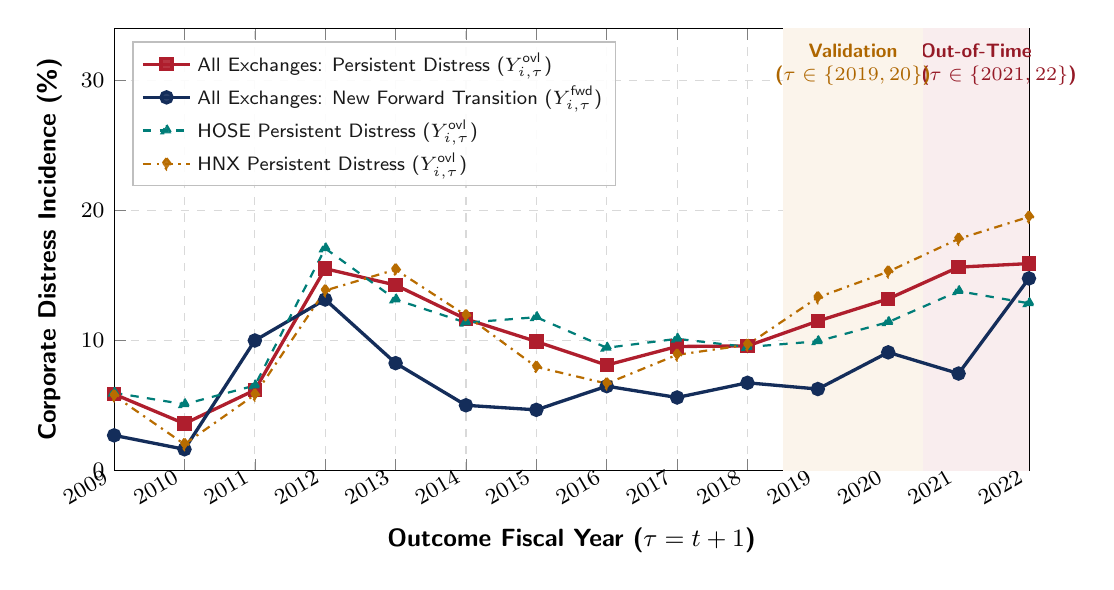
\begin{tikzpicture}
\begin{axis}[
    width=13.2cm,
    height=7.2cm,
    xlabel={\textbf{Outcome Fiscal Year ($\tau = t + 1$)}},
    ylabel={\textbf{Corporate Distress Incidence (\%)}},
    xmin=2009, xmax=2022,
    ymin=0, ymax=34,
    xtick={2009,2010,2011,2012,2013,2014,2015,2016,2017,2018,2019,2020,2021,2022},
    xticklabels={2009,2010,2011,2012,2013,2014,2015,2016,2017,2018,2019,2020,2021,2022},
    xticklabel style={font=\footnotesize, rotate=30, anchor=east},
    yticklabel style={font=\footnotesize},
    label style={font=\small\sffamily},
    grid=both,
    grid style={dashed, gray!30},
    legend style={at={(0.02,0.97)}, anchor=north west, font=\scriptsize\sffamily, fill=white, fill opacity=0.9, draw=gray!50},
    legend cell align={left},
    clip=false
]

% Shaded Test Regime (2021-2022)
\fill[crimson!8] (axis cs:2020.5,0) rectangle (axis cs:2022,34);
\node[font=\scriptsize\sffamily\bfseries, color=crimson!85!black, align=center] at (axis cs:2021.25,31.2) {Out-of-Time\\Test ($\tau \in \{2021,22\}$)};

% Shaded Val Regime (2019-2020)
\fill[amber!8] (axis cs:2018.5,0) rectangle (axis cs:2020.5,34);
\node[font=\scriptsize\sffamily\bfseries, color=amber!85!black, align=center] at (axis cs:2019.5,31.2) {Validation\\($\tau \in \{2019,20\}$)};

\addplot[color=crimson, very thick, mark=square*, mark size=2pt] coordinates {
    (2009,5.88) (2010,3.61) (2011,6.19) (2012,15.52) (2013,14.26) (2014,11.65) (2015,9.92) (2016,8.11) (2017,9.54) (2018,9.58) (2019,11.49) (2020,13.20) (2021,15.64) (2022,15.91)
};
\addlegendentry{All Exchanges: Persistent Distress ($Y_{i,\tau}^{\text{ovl}}$)}

\addplot[color=navy, very thick, mark=*, mark size=2pt] coordinates {
    (2009,2.71) (2010,1.64) (2011,10.00) (2012,13.15) (2013,8.26) (2014,5.02) (2015,4.67) (2016,6.49) (2017,5.62) (2018,6.75) (2019,6.27) (2020,9.09) (2021,7.46) (2022,14.77)
};
\addlegendentry{All Exchanges: New Forward Transition ($Y_{i,\tau}^{\text{fwd}}$)}

\addplot[color=teal, thick, dashed, mark=triangle*, mark size=2pt] coordinates {
    (2009,5.98) (2010,5.10) (2011,6.54) (2012,17.08) (2013,13.15) (2014,11.37) (2015,11.79) (2016,9.44) (2017,10.13) (2018,9.50) (2019,9.94) (2020,11.41) (2021,13.79) (2022,12.86)
};
\addlegendentry{HOSE Persistent Distress ($Y_{i,\tau}^{\text{ovl}}$)}

\addplot[color=amber!90!black, thick, dashdotted, mark=diamond*, mark size=2pt] coordinates {
    (2009,5.77) (2010,2.03) (2011,5.83) (2012,13.84) (2013,15.45) (2014,11.93) (2015,7.97) (2016,6.69) (2017,8.90) (2018,9.67) (2019,13.31) (2020,15.29) (2021,17.81) (2022,19.50)
};
\addlegendentry{HNX Persistent Distress ($Y_{i,\tau}^{\text{ovl}}$)}

\addplot[color=purple, thick, densely dotted, mark=pentagon*, mark size=2pt] coordinates {
    
};
\addlegendentry{UPCOM Persistent Distress ($Y_{i,\tau}^{\text{ovl}}$)}

\end{axis}
\end{tikzpicture}
\end{document}
